\subsubsection{pr07}
\label{subsubsec:pr07}
The obtained results were the following:
{
\renewcommand{\arraystretch}{2}
\begin{longtable}[h]{| c | c | c | c | c |}
    \hline
    \textbf{Failures} & \multicolumn{3}{c}{Time limit} & \\
    \hline
    \textbf{Search strategy} & \textbf{\textit{30 sec}} & \textbf{\textit{1 min}} & \textbf{\textit{2 min}} & \textbf{\textit{5 min}} \\
    \hline
    \endhead
    default search                                         & 22.048 &  46.013 & 115.991 & 503.148 \\
    \hline
    domWdeg, random                                        & 39.907 & 114.655 & 256.773 & 664.906 \\
    \hline
    domWdeg, random, Luby restart L=250                    & 18.135 &  50.513 & 118.099 & 339.991 \\
    \hline
    \textit{domWdeg, random, Luby restart L=250, LNS 85\%} &   114 &    242 &   1.152 &  48.390 \\
    \hline
    domWdeg, random, Luby restart L=250, LNS 15\%          &  8.780 &  23.470 &  89.865 & 400.126 \\
    \hline
    first fail, min                                        & 28.313 &  83.192 & 185.166 & 555.740 \\
    \hline
\end{longtable}
}
\begin{figure}[H]
    \centering
    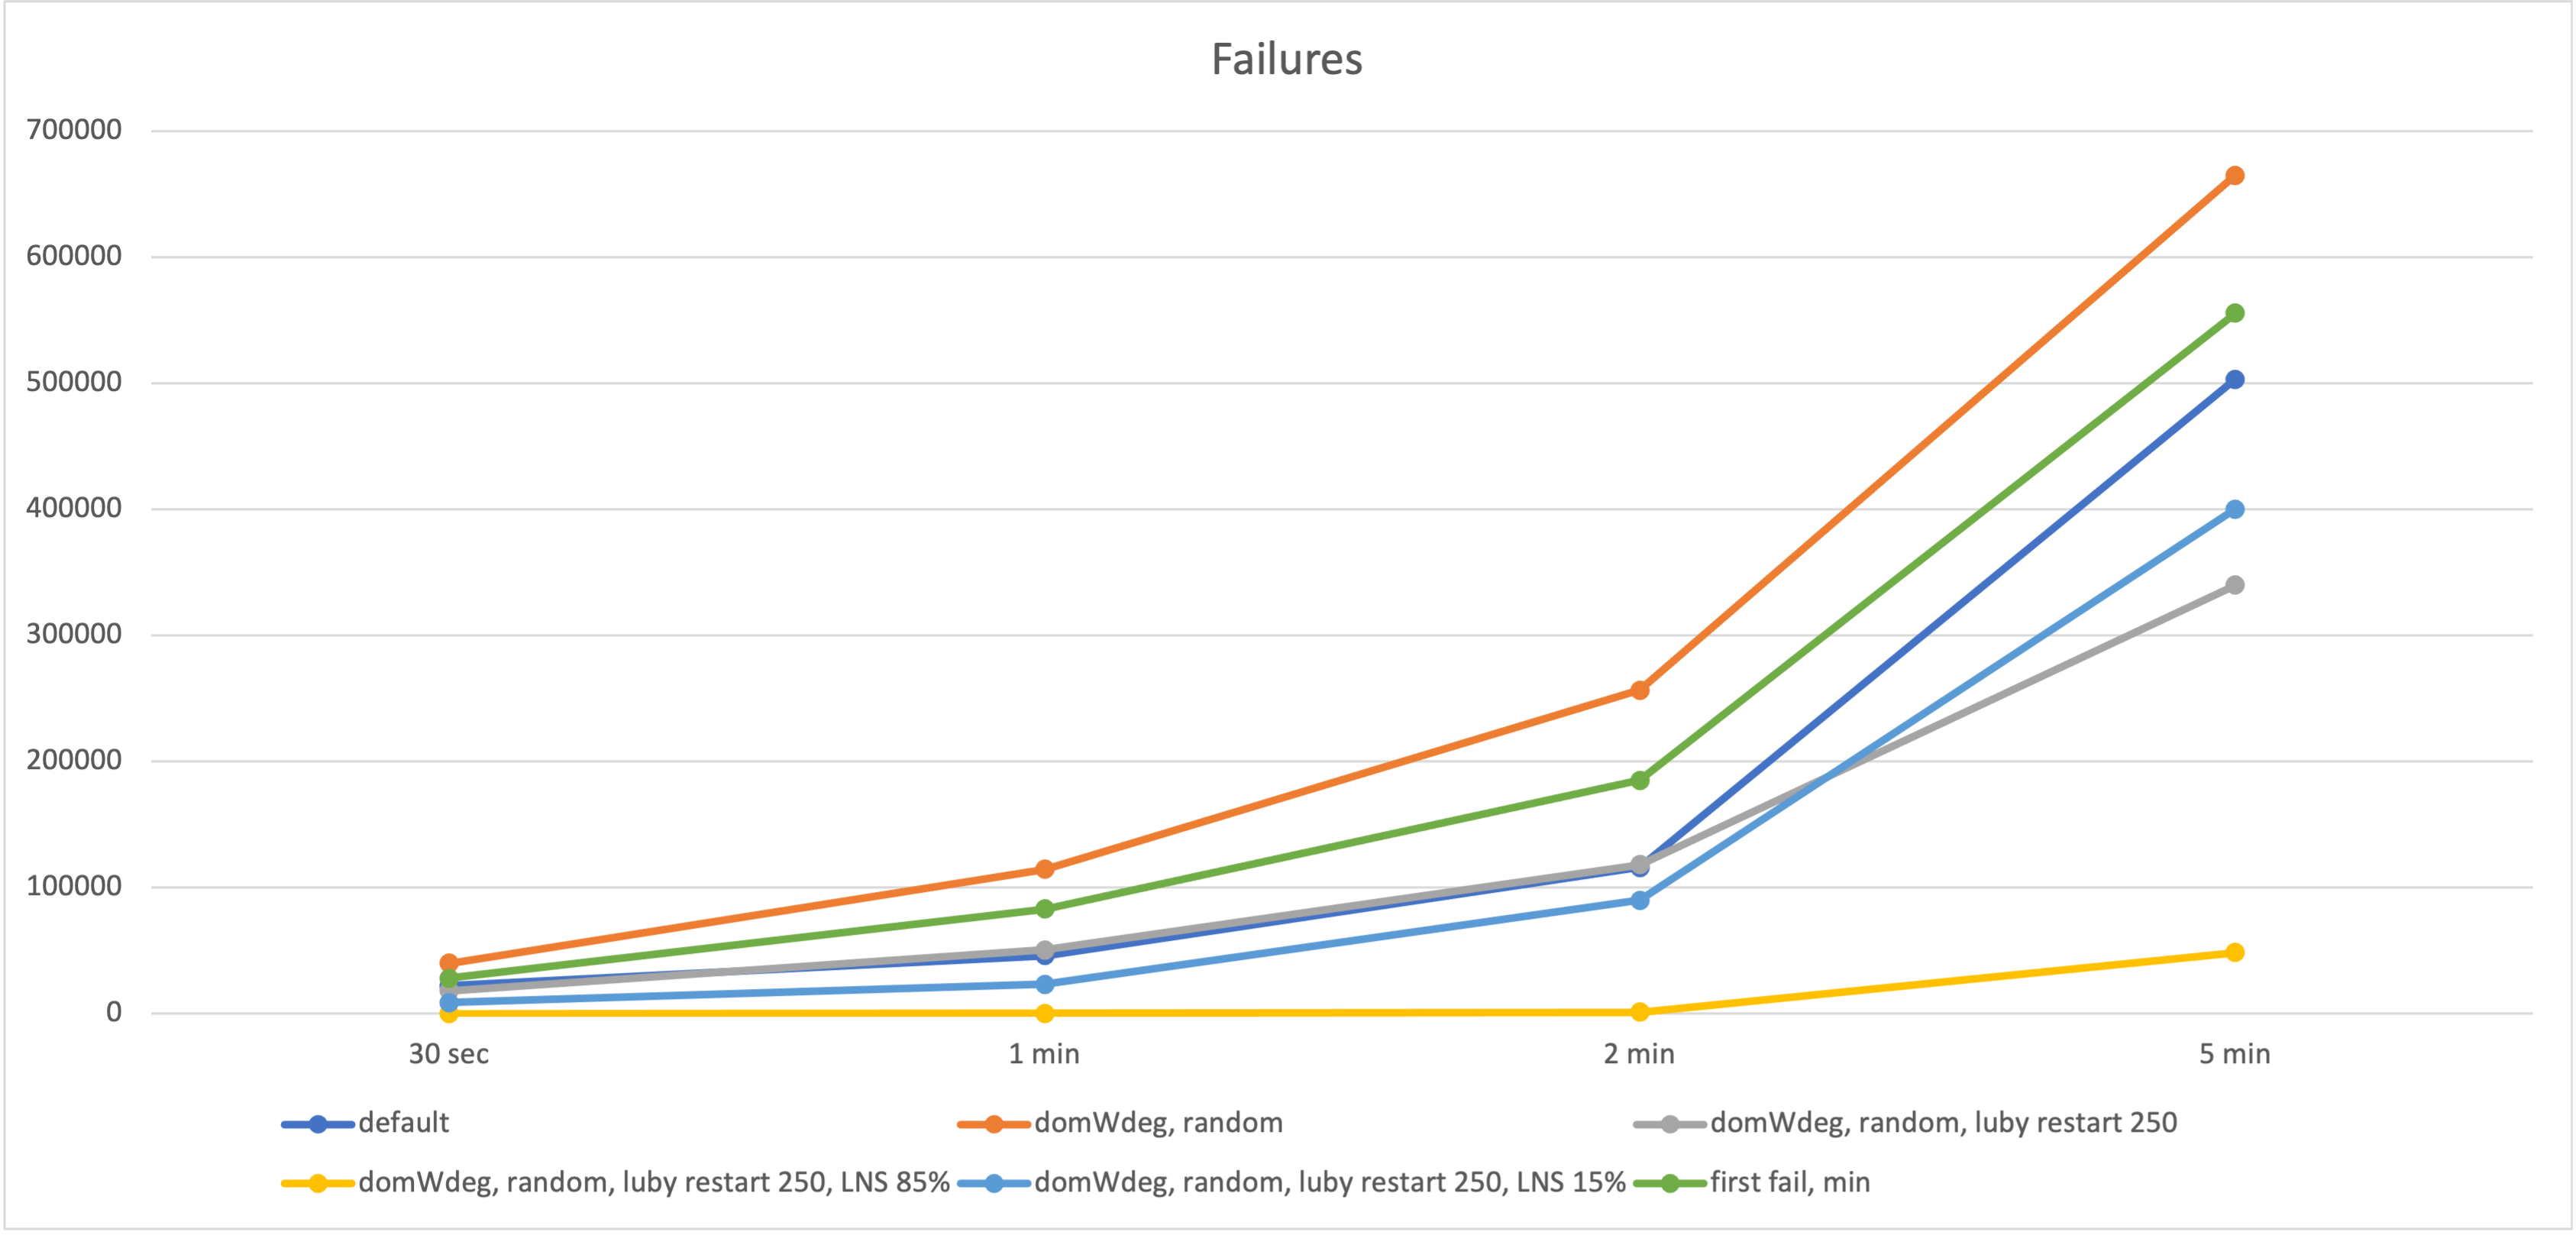
\includegraphics[width=0.8\columnwidth]{../graphs/pr07-failures.png}
    \caption{Failures graph for \textbf{pr07}.}
\end{figure}

{
\renewcommand{\arraystretch}{2}
\begin{longtable}[h]{| c | c | c | c | c |}
    \hline
    \textbf{Objective function} & \multicolumn{3}{c}{Time limit} & \\
    \hline
    \textbf{Search strategy} & \textbf{\textit{30 sec}} & \textbf{\textit{1 min}} & \textbf{\textit{2 min}} & \textbf{\textit{5 min}} \\
    \hline
    \endhead
    default search                                         & 49.388.330 & 47.598.050 & 45.738.130 & 45.434.580 \\
    \hline
    domWdeg, random                                        & 52.560.080 & 52.560.080 & 52.560.080 & 51.534.010 \\
    \hline
    domWdeg, random, Luby restart L=250                    & 51.466.840 & 50.774.060 & 47.193.750 & 47.193.750 \\
    \hline
    \textit{domWdeg, random, Luby restart L=250, LNS 85\%} & 52.650.040 & 49.037.820 & 37.230.030 & 17.390.370 \\
    \hline
    domWdeg, random, Luby restart L=250, LNS 15\%          & 53.260.710 & 49.568.660 & 48.247.640 & 47.041.040 \\
    \hline
    first fail, min                                        & 48.175.380 & 48.039.940 & 47.949.990 & 47.949.990 \\
    \hline
\end{longtable}
}
\begin{figure}[H]
    \centering
    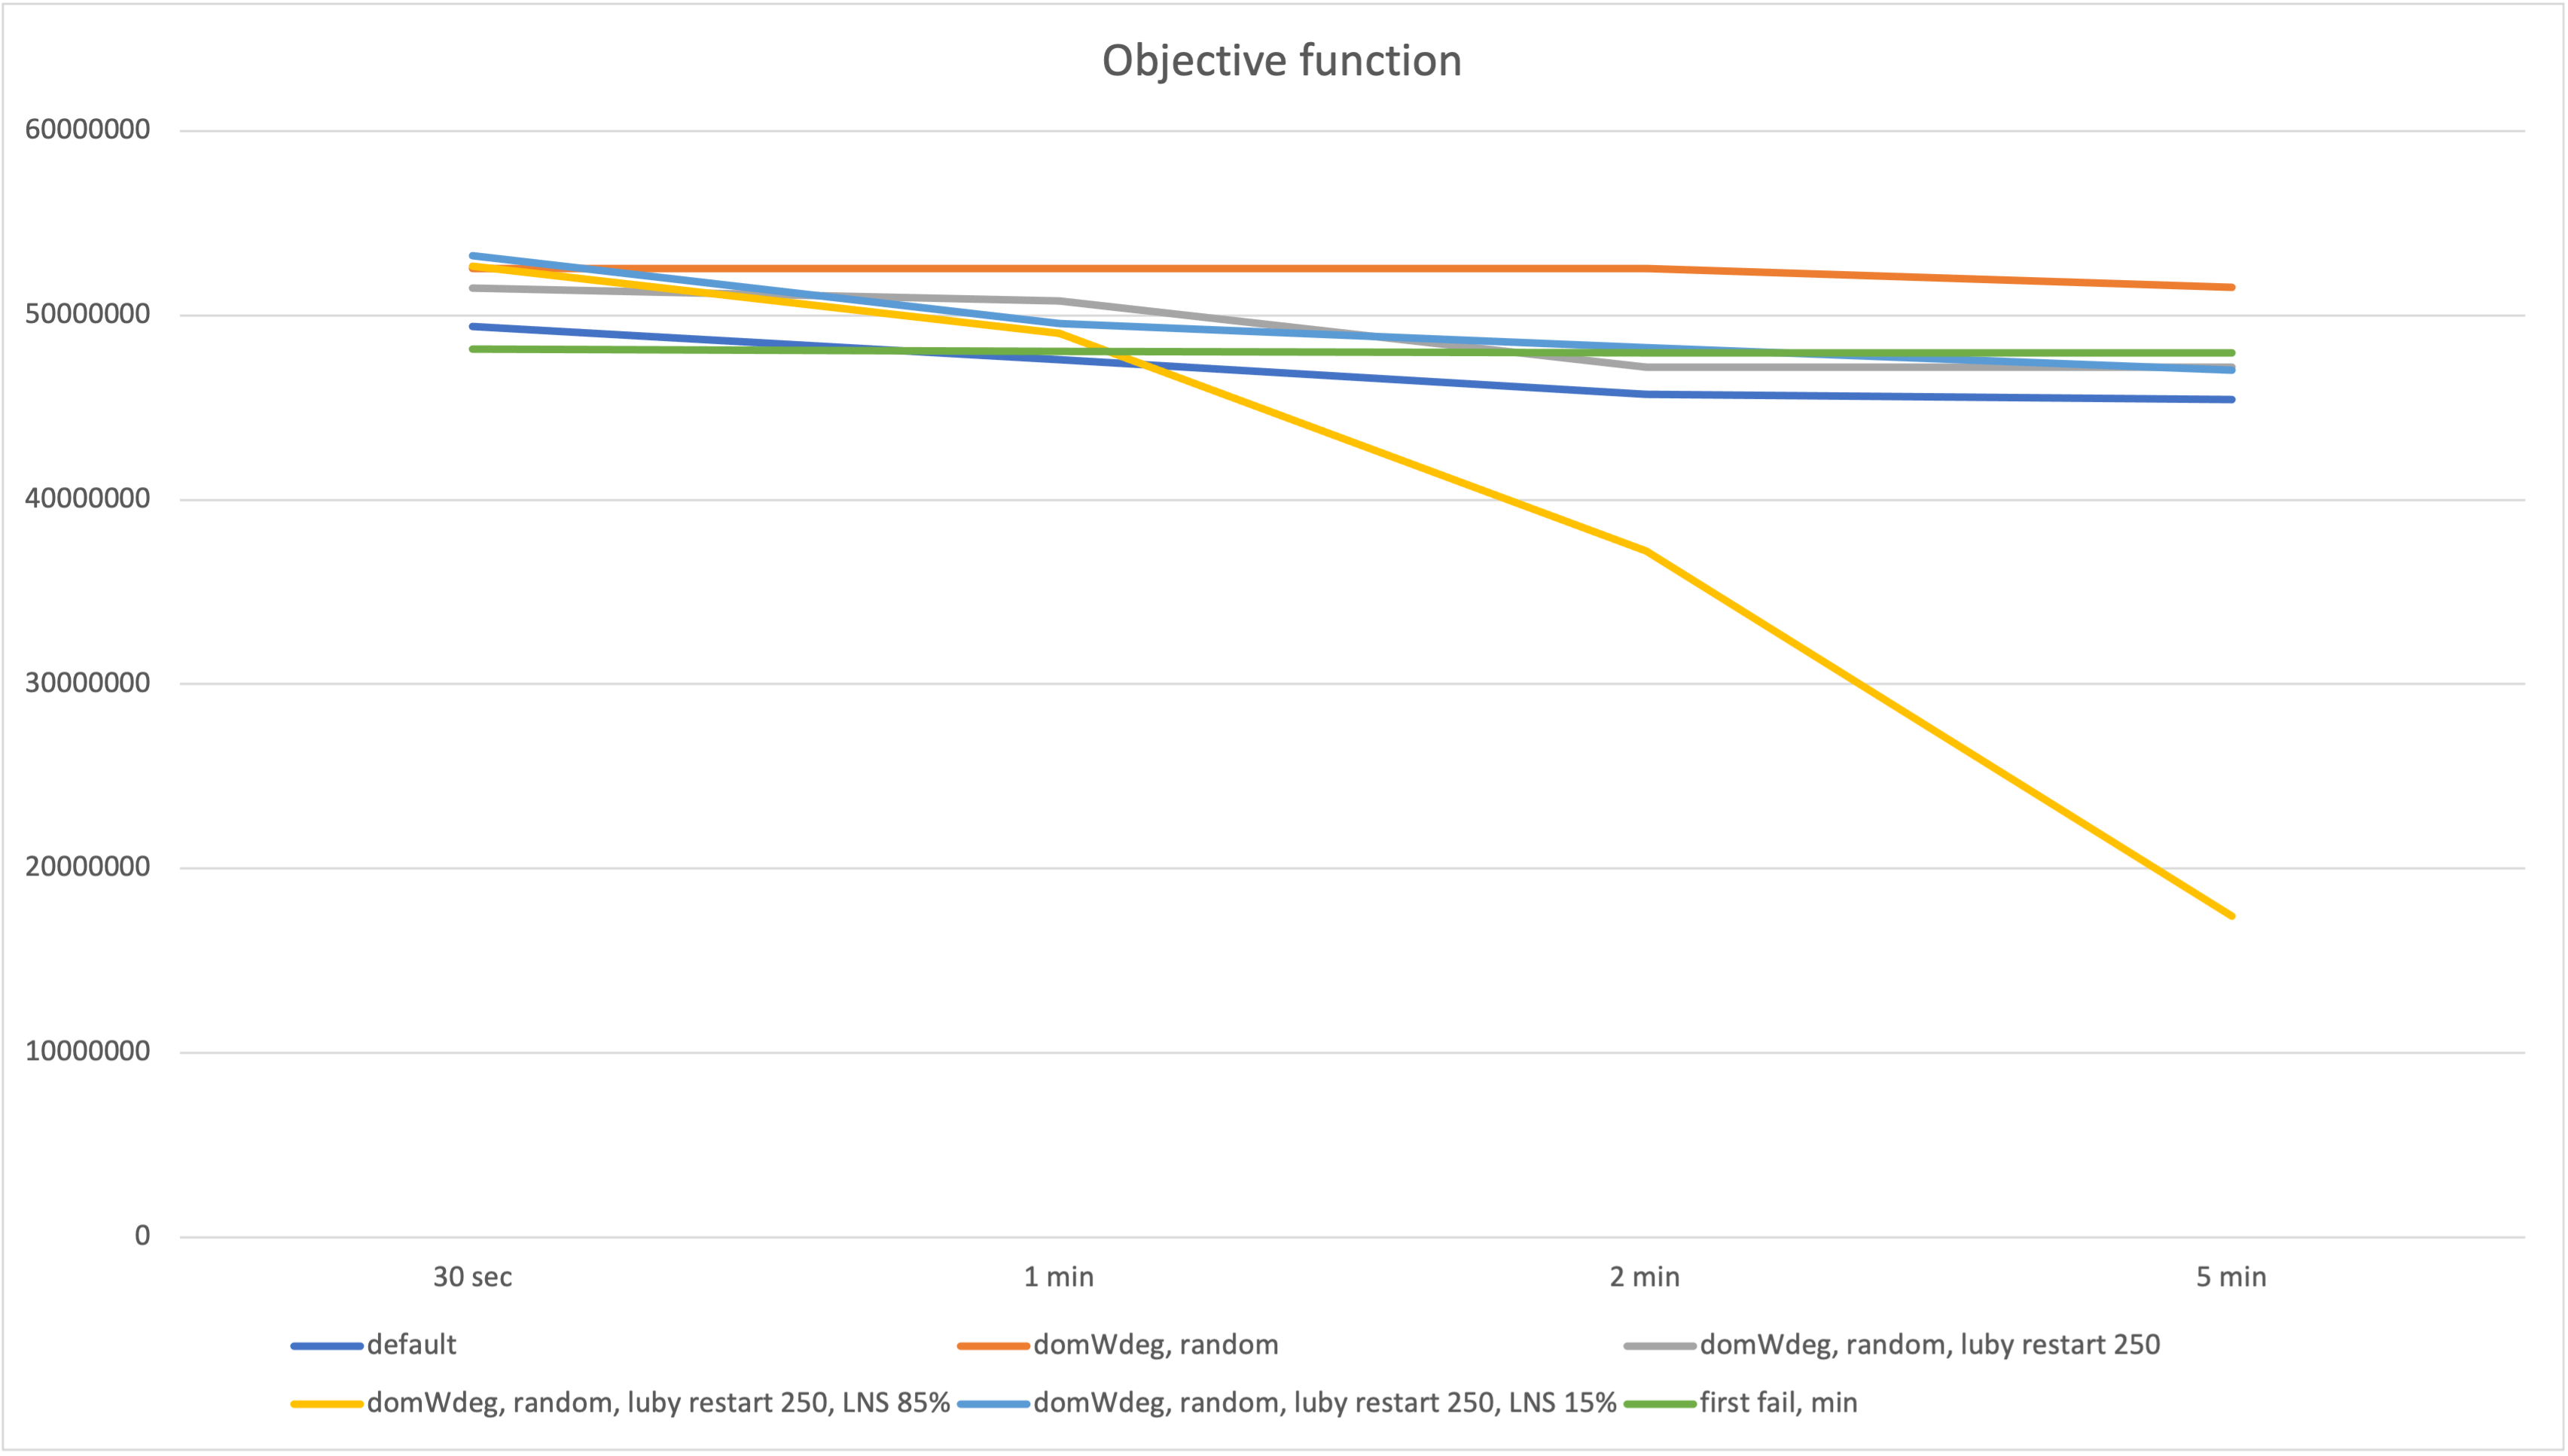
\includegraphics[width=0.8\columnwidth]{../graphs/pr07-objf.png}
    \caption{Objective functions graph for \textbf{pr07}.}
\end{figure}

{
\renewcommand{\arraystretch}{2}
\begin{longtable}[h]{| c | c | c | c |}
    \hline
    \textbf{Weights} & \textbf{Objective function} & \textbf{Total distance} & \textbf{Used vehicles} \\
    \hline
    \endhead
    $\alpha = 10, \beta = 0$ & 22.938.800 & 2.293.880 & 7 \\
    \hline
    $\alpha = 7, \beta = 3$  & 15.124.836 & 2.160.687 & 9 \\
    \hline
    $\alpha = 5, \beta = 5$  & 10.803.480 & 2.160.687 & 9 \\
    \hline
    $\alpha = 3, \beta = 7$  &  6.545.857 & 2.181.936 & 7 \\
    \hline
    $\alpha = 0, \beta = 10$ &         40 & 5.063.819 & 4 \\
    \hline
\end{longtable}
}
\begin{figure}[H]
    \centering
    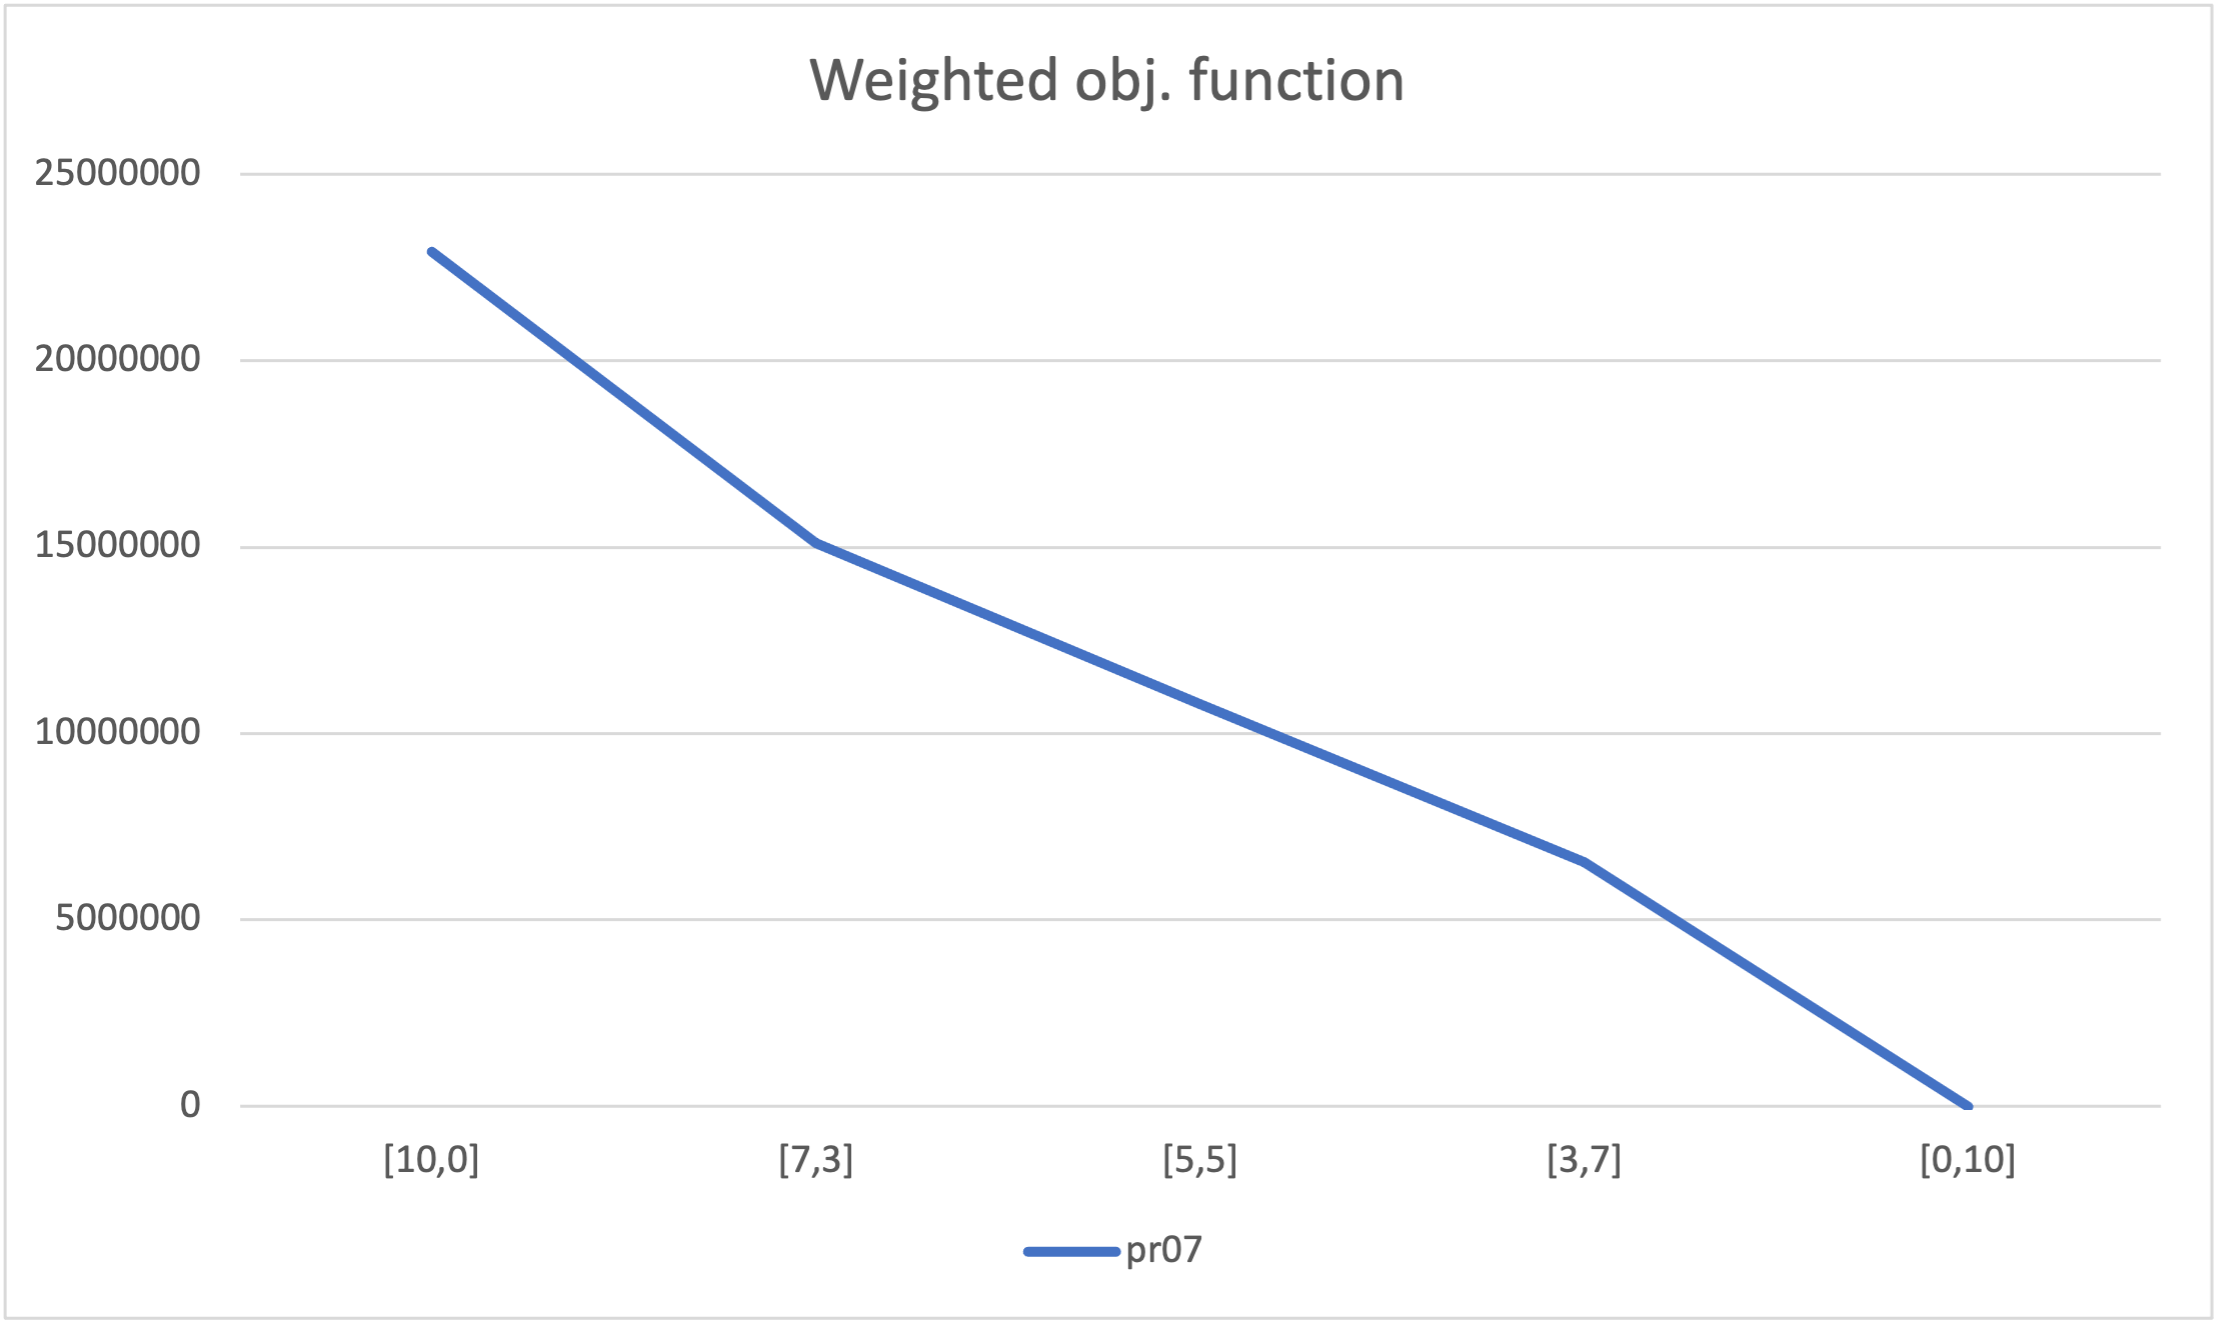
\includegraphics[height=0.25\textheight]{../graphs/pr07-wobjf.png}
    \caption{Weighted objective functions graph for \textbf{pr07}.}
\end{figure}

\begin{figure}[H]
    \centering
    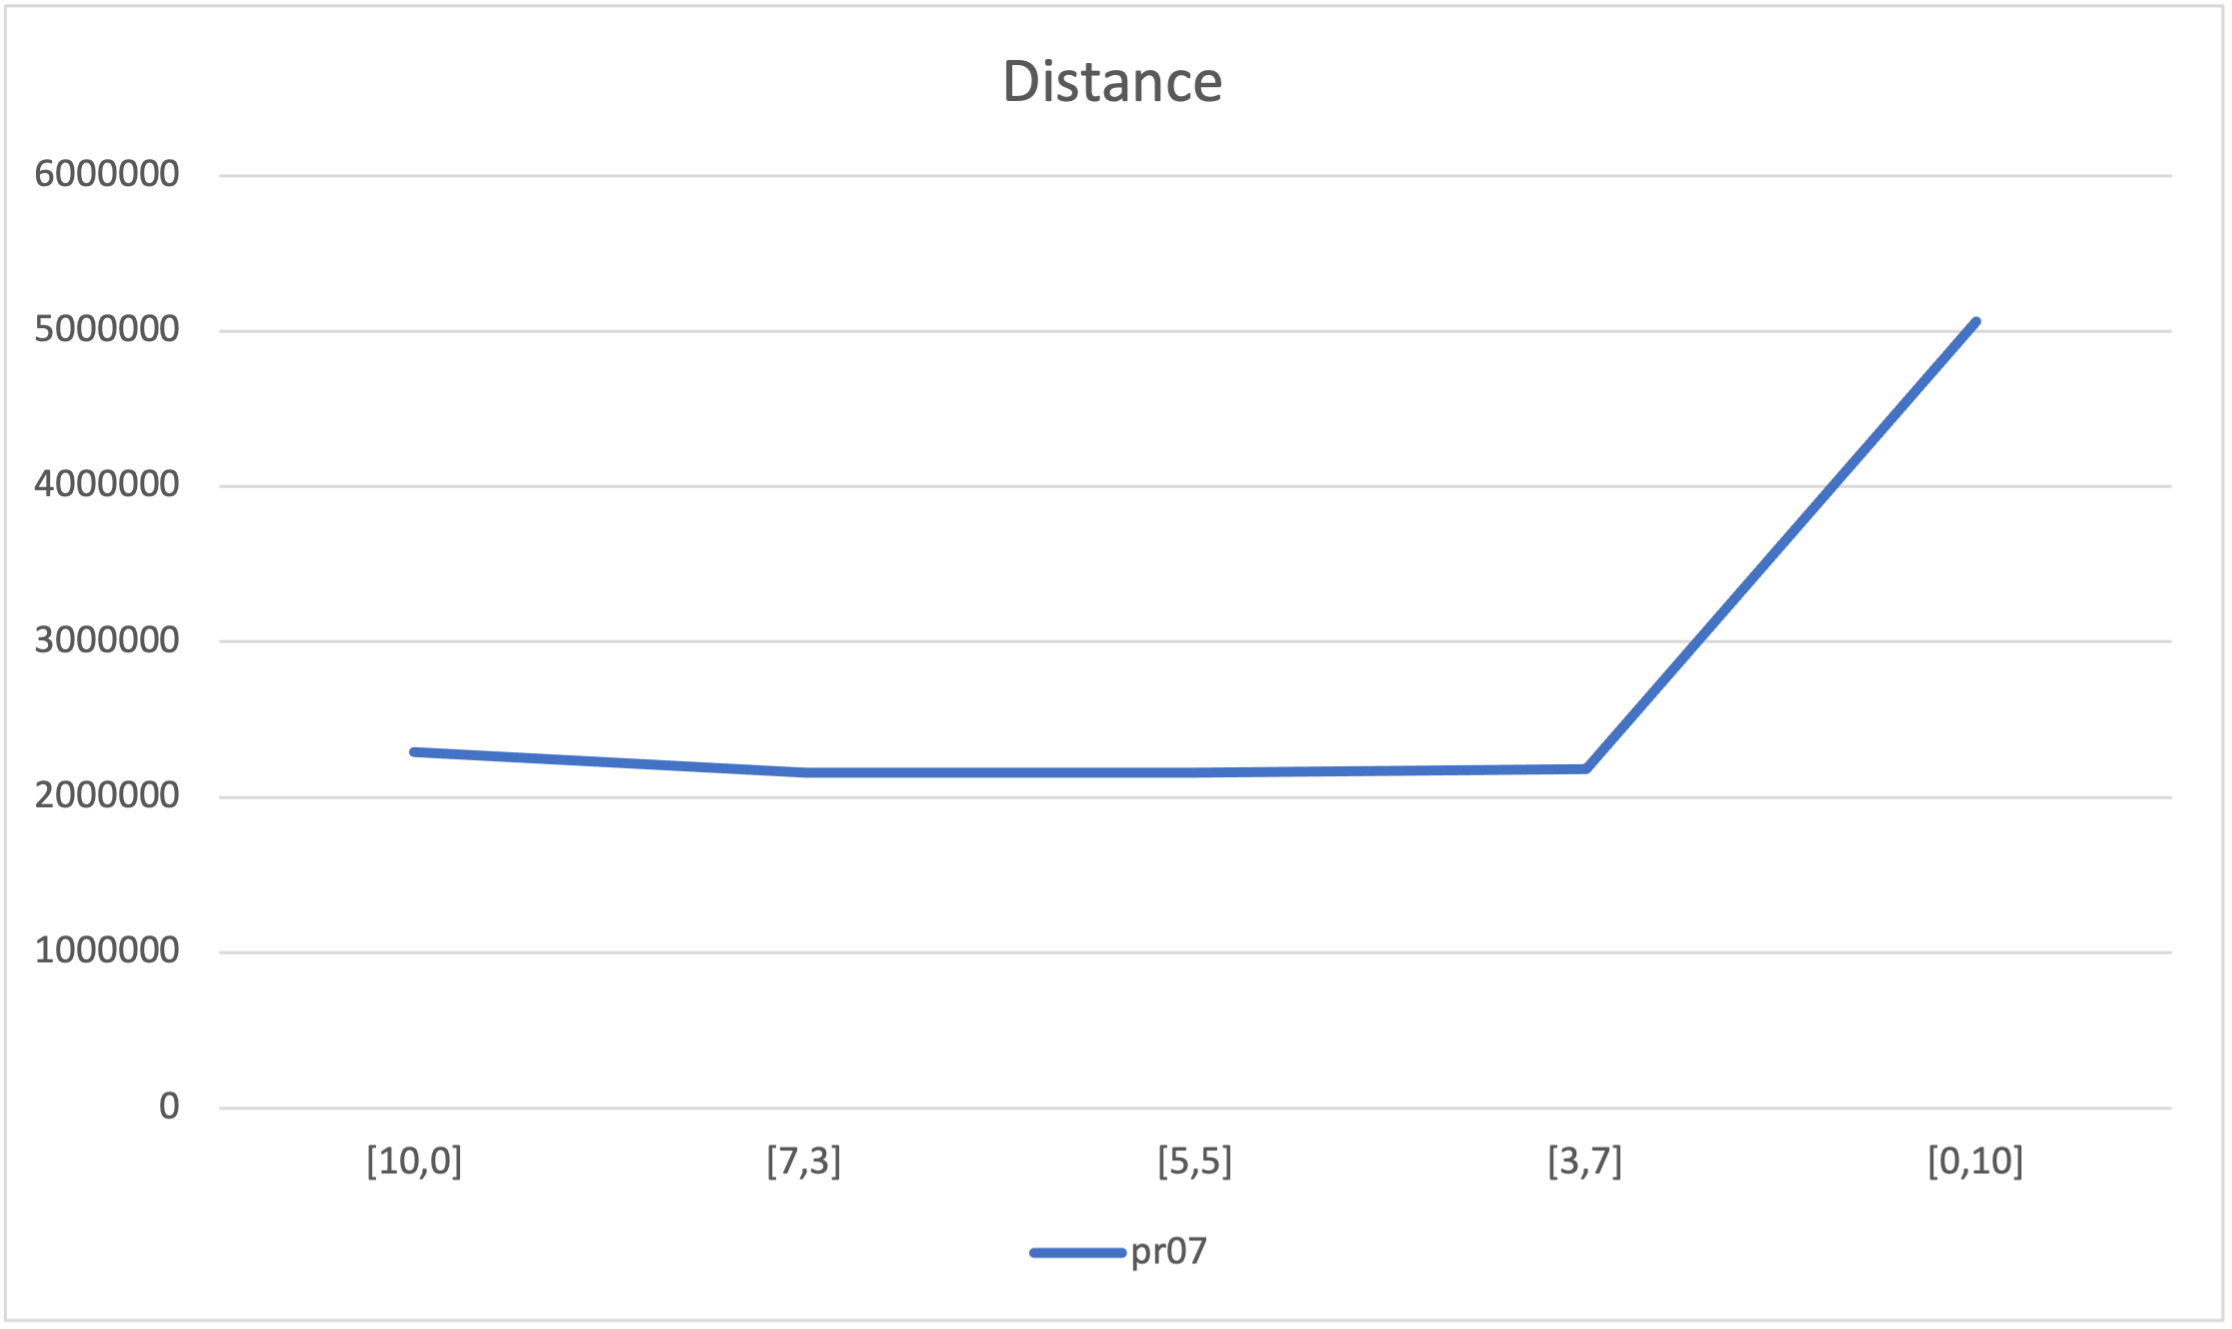
\includegraphics[height=0.25\textheight]{../graphs/pr07-distance.png}
    \caption{Distances graph for \textbf{pr07}.}
\end{figure}

\begin{figure}[H]
    \centering
    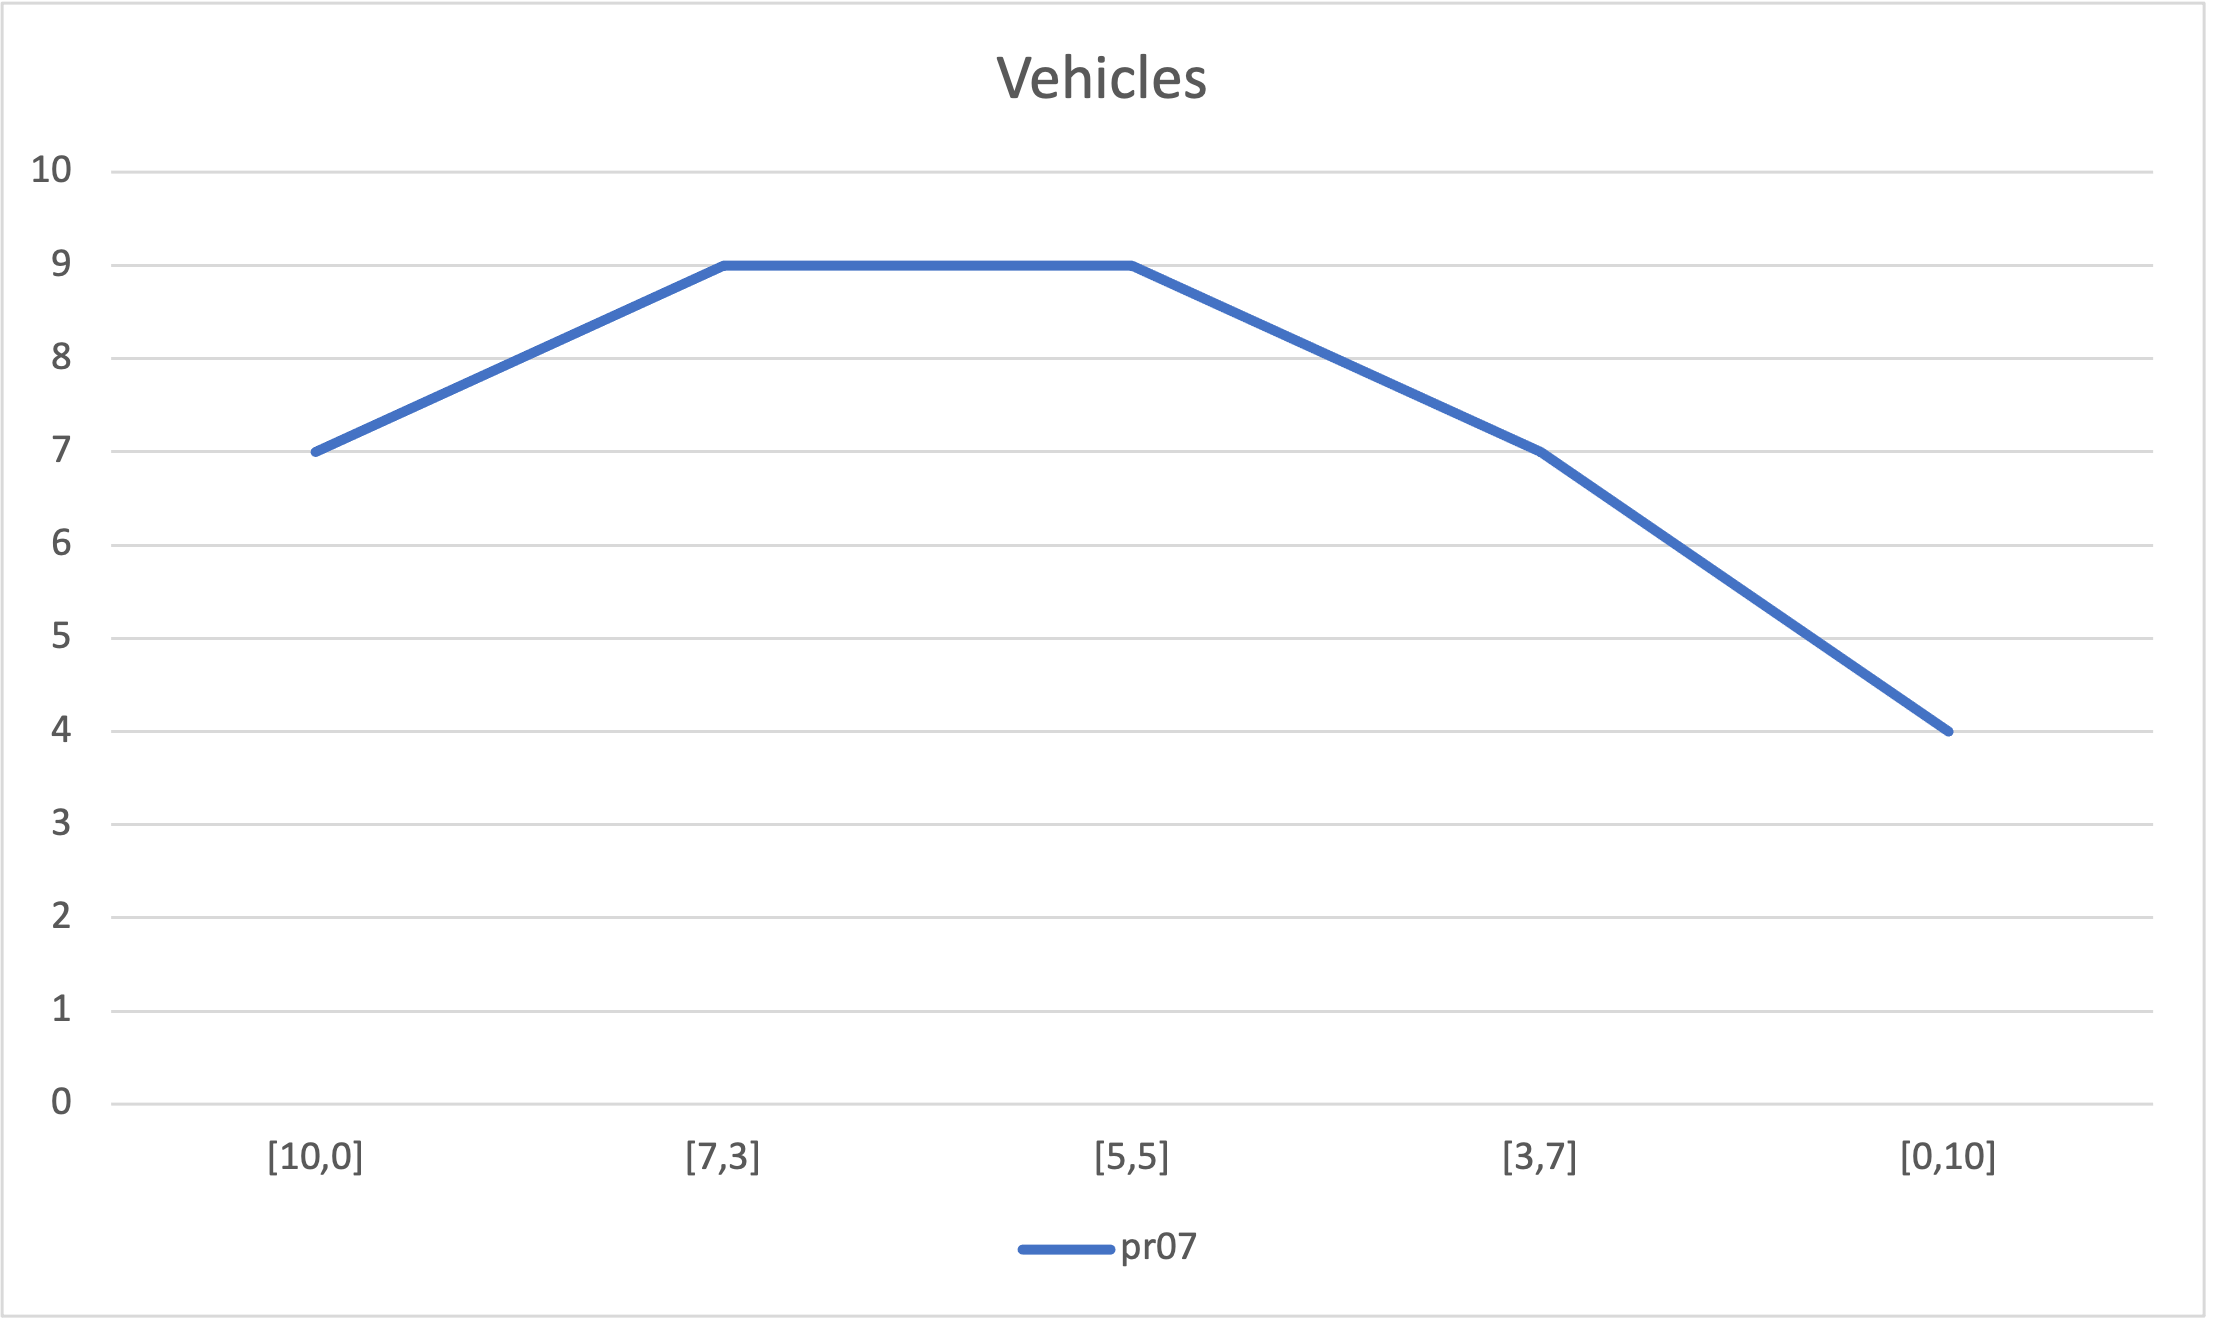
\includegraphics[height=0.25\textheight]{../graphs/pr07-vehicles.png}
    \caption{Vehicles used graph for \textbf{pr07}.}
\end{figure}

\newpage
